\documentclass{article}

\usepackage{enumerate}
\usepackage[margin=1.5in]{geometry}
\usepackage{tikzit}
\usepackage{tikz-cd}
\usepackage{amsthm}
\usepackage{amsmath}
\usepackage{amsfonts}
\usepackage{braket}
\usepackage{mathtools}


\newtheorem{theorem}{Theorem}[section]
\newtheorem{lemma}{Lemma}[section]
\newtheorem{corollary}{Corollary}[section]
\newtheorem{conjecture}{Conjecture}[section]
\newtheorem{proposition}{Proposition}[section]

\theoremstyle{definition}
\newtheorem*{definition}{Definition}


\graphicspath{ {./images/} }
\numberwithin{figure}{section}
\setcounter{section}{-1}



\title{The Algebraic Theory\\ of \\ Topological Quantum Information}
\author{by Milo Moses}

\date{\textit{California Institute of Technology} \\ [2ex] \today}


\begin{document}


\maketitle

\newcommand{\wind}{\mathrm{wind}}
\newcommand{\Free}{\mathrm{Free}}
\newcommand{\Sym}{\mathrm{Sym}}


\newcommand{\RR}{\mathbb{R}}
\newcommand{\ZZ}{\mathbb{Z}}
\newcommand{\QQ}{\mathbb{Q}}
\newcommand{\CC}{\mathbb{C}}
\newcommand{\SO}{\mathrm{SO}}


\newcommand{\0}{\left|0\right>}
\newcommand{\1}{\left|1\right>}



\begin{abstract}
This book aims to give a comprehensive account of the algebraic theory of topological quantum information. It is intended to be accessible both to mathematicians unfamiliar with quantum mechanics and theoretical physicists unfamiliar with category theory. Additionally, this text should make a good reference for working researchers in the field. A primary focus of this text is the balancing of powerful algebraic generalities with concrete examples, principles, and applications.
\end{abstract}


\newpage

\tableofcontents

\newpage


\section{Preface}
\label{Preface}

This book is a mathematical treatment of topological quantum information, with a focus on formal algebraic aspects and a special eye towards topological quantum computation. This manuscript began as an extended set of notes from a course on topological quantum field theory given by Zhenghan Wang in the winter of 2022 at UC Santa Barbara. Through his courses, his private tutoring, and his reccomendations, Zhenghan took me from a state of almost complete ignorance of mathematical physics to being a young researcher in the field. I am greatly emdebted to him for this, and it is certain that this book would not have existed without his guidance - he richly deserves of my apple.

Great pains have been taken to make this book as pedagogical and accessable as possible. The hope is that it should be readable by both mathematicians unfamilar with quantum mechanics as well as theoretical physicists unfamiliar with category theory. A primary focus of this text is the balancing of powerful algebraic generalities with concrete examples, principles, and applications. The prerequisites for this book are a undergraduate-level understanding of topology, abstract algebra, as well as a popular-science level of familarity with quantum mechanics.

There are already many great references to learn aspects of the material covered in this book. An excellently written and relatively complete book on topological quantum information from the perspective of a physicist is Steven Simon's text \cite{simon2023topological}. Simon's book is very algebraic, but does \textit{not} include any category theory. The main references for the relevant category theory are Bakalov-Kirillov \cite{bakalov2001lectures} and Etingof-Gelaki-Nikshych-Ostrik \cite{etingof2016tensor}. While both excellent texts, they both have notable shortcomings for learning topological quantum information. Bakalov-Kirillov was written in 2001, making it very outdated. Etingof-Gelaki-Nikshych-Ostrik is modern, but makes no connections to physics and does not use the language of string diagrams. The manuscript most similar to this one is Kong-Zhang's preprint \cite{kong2022invitation}. We distinguish ourself from Kong-Zhang by our different choice of topics, our different choice of treatment, and our extended scope. Other relevant books and review articles include Wang's monograph \cite{wang2010topological}, Kauffman-Lomonaco's quantum topology themed review \cite{kauffman2009topological}, and Bartlett's topological quantum field theory PhD thesis \cite{bartlett2005categorical}.

The structure of this book is as follows.

\begin{enumerate}
\item Chapter \ref{overview} (Overview): This chapter gives an overview of the subject, and aquaints the reader with the important principles of topological quantum computation. Section \ref{conceptual introduction} gives a non-technical primer on the subject, including motivation, applications, and history. Section \ref{technical introduction} covers topological \text{classical} information, as a playing ground in which to highlight the important principles of the field. This includes a crash-course on the relevant toplogy, which may be unfamilar to some readers.

\end{enumerate}

\newpage

\section{Overview}
\label{overview}

\subsection{Conceptual introduction}
\label{conceptual introduction}

\subsubsection{Motivation and applications}

I will take as a definition \textit{topological quantum information} to be the study of information in topological quantum systems. A topological quantum system is some mathematical or physical system which is in a fundamental sense described by the mathematics of both quantum mechanics and topology. The term \textit{quantum system} here is used in contrast to \textit{classical system}. The flow of current through a conducting copper wire is described perfectly well by classical electromagnetism, whereas the flow of current through a superconducting niobium-titanium wire necessarily requires quantum mechanics for its description.

The term \textit{topological system} is used in contrast to \textit{geometric systems}, though the term “geometric system” is a nonstandard one. In a geometric system, measurable quantities and phenomena depend on quantitative local aspects of the system - the distance between wires, the exact shape of some sample, or the curvature of some component. In a topological system, measurable quantities and phenomena depend only on qualitative global aspects of the system - whether two wires cross or not, whether a sample is connected or not, whether a component curves into a ball or has a boundary.

I say that this book is about “topological quantum information” and not “topological quantum systems” for two reasons. The first is to highlight the fact that topological quantum systems \textit{do} have local geometric descriptions, which we will mostly be ignoring them in favor of focusing on their global topological properties. The beauty of topological systems lies exactly in the fact that this global perspective retains all the essential information in the system. The second reason I use the term \textit{information} is to highlight this book’s eye towards topological quantum computing. 

Since Peter Shor’s 1994 discovery of an efficient factoring algorithm on quantum computers \cite{shor1994algorithms}, the primary goal of quantum information theorists has been to harness quantum information sufficiently well so that it can be used to make an efficient scalable quantum computer. One of the major hurdles in achieving this goal is that quantum information is \textit{fragile}. Small amounts of noise coming from nearby electromagnetic fields or imperfections in experimental devices are often enough to affect the information being stored, resulting in \textit{errors} in the computation. In the early days of quantum computing it was not clear whether there was any way around this problem. Perhaps the inherent fragility of quantum information would make quantum computation impossible. This turned out to be false.

The beautiful observation is that errors are not nearly as catastrophic in \textit{topological} quantum systems. Errors are typically local, and by definition the information topological systems does not depend on local properties. Hence, under suitable conditions, topological systems are naturally error resistant! In the same way that invariants of topological spaces are supposed to be invariant under deformations in pure mathematics, information in topological systems is invariant under errors in mathematical physics. Hence, to solve the problem of noise all one has to do is make a \textit{topological} quantum computer! This observation was made in 1997 and is due independently to Alexei Kitaev and Michael Freedman \cite{kitaev2003fault, freedman1998p}. Since then topological quantum computing has grown and evolved, finding its way into almost every modern proposal for fault-tolerant quantum computing.

The first approach to topological quantum computing is to use a physical material, some literal condensed collection of atoms, which naturally behaves as a topological quantum system. These exist and have been studied for a long time. For instance, a two dimensional sheet of graphene behaves topologically when it is subjected to low temperatures ($\approx$5 degrees Kelvin) and large magnetic fields ($\approx$15 Teslas) \cite{bolotin2009observation}. Topological quantum materials which can be used to make scalable quantum computers require intricate experiments to operate, which has been the most prominent roadblock in this approach.

The second approach to topological quantum computing is to artificially construct a topological system within a geometric one. The function of a quantum computer, almost by definition, is to simulate quantum systems. In particular, it can simulate \textit{topological} quantum systems. Since topological systems are resistant to local errors, this means that the original computer which is simulating the topological system will itself become resistant to local noise! This works exactly as described as long as the simulation itself is local, that is, local effects in the original system correspond to local effects in the simulated system. This technique of simulating a topological system to inherit its error-resistant properties is known as \textit{topological quantum error correction}. The advantage of this approach is that it works on any hardware available. The disadvantage is that to perform useful computations one must pass through the topological quantum error correction. The additional layer adds a hefty amount of overhead, which can eat up the majority of runtime and resources. It is for this reason that \textit{efficient} topological quantum error correction is an important and active area of research.

\[\begin{tikzcd}
	& \begin{array}{c} \substack{\text{topological}\\ \text{quantum}\\\text{materials}} \end{array} \\
	\begin{array}{c} \substack{\text{topological} \\ \text{quantum} \\ \text{information}} \end{array} \\
	& \begin{array}{c} \substack{\text{topological}\\\text{quantum}\\ \text{error correction}} \end{array}
	\arrow["\begin{array}{c} \substack{\text{intrinsic}\\\text{realization}} \end{array}", from=2-1, to=1-2]
	\arrow["\begin{array}{c} \substack{\text{local}\\\text{simulation}} \end{array}"', from=2-1, to=3-2]
\end{tikzcd}\]

Of course, the above discussion presents only one motivation for topological quantum information and only one example of an application. Topological quantum materials open a whole world of potential applications, and it seems they may play an important role in the techonologies of the future \cite{ramirez2020dawn}. Some proposed applications include processing classical information using topological defects in magnetic devices (with the end goal of making high-speed low-energy transmissions) \cite{marrows2021perspective, vsmejkal2018topological}, creating highly sensitive photodetectors (with the end goal of making night-vision goggles or sensors) \cite{chan2017photocurrents}, creating technolgies with high thermoelectric effect (with the end goal of making efficient fridges or electric generators) \cite{skinner2018large}, creating highly-efficient transistors \cite{fuhrer2021proposal}, and engineering tiny electrical components \cite{viola2014hall, placke2017model}. 

This breadth of potential applications is due in part to the number of different types of topological materials which have been discovered or theorized. This includes quantized Hall states \cite{von202040}, topological insulators \cite{hasan2010colloquium}, fractional Chern insulators \cite{regnault2011fractional}, Weyl/Dirac semimetals \cite{armitage2018weyl}, and topological superconductors \cite{sato2017topological}. The contents of this book certainly do not provide the entire picture for any of these materials. However, the hope is that it gives a picture of the algebraic structures within them, hence helping readers think both concretely and conceptually about these materials and their applications.

\subsubsection{Mathematical picture}

The term \textit{topological quantum system} is broad. To get a rigorous mathematical subject, we will focus on a specific type of topological quantum system known as a \textit{topologically ordered} quantum system. Topological order is much more precise, though there are still conflicting definitions in the literature. Specifically, I will be focusing on \textit{(2+1)-dimensional} topological order. Here, I am using the physicist convention of using (2+1)D to refer to two space dimensions and one time dimension. That is, I will be discussing a locally flat topologically ordered system. For example, a single sheet of graphene at low temperatures and large magnetic fields can exhibit a form of (2+1)D topological order, and any quantum computer running topological quantum error correction can also exhibits a form of (2+1)D topological order.

\begin{center}
\fbox{All systems in this book are two-dimensional unless stated otherwise.}
\end{center}

The naive mathematical description of topological order is \textit{topological quantum field theory}. In a sense, we can \textit{define} a topologically ordered system to be a system which admits a description in terms of topological quantum field theory. Geometric quantum systems require non-topological quantum field theory to describe.

While they are useful in many contexts, topological quantum field theories do have several difficulties associated with them. The most prominent of which is that their definition requires a large amount of essentially redundant data. This makes them hard to construct, inaccessible to computational methods, and opaque in their realizations of important phenomena. One solution to this problem is to dig down to the core algebraic data lying within topological quantum field theories. This algebraic data contains far less redundancy than the original topological quantum field theory. This makes the algebraic data thus easier to construct, more accessible to computational methods, and more clear in its realization of important phenomena. The algebraic structure which houses the algebraic data of a (2+1)D topological quantum field theory is known as a \textit{modular tensor category}. These algebraic structures are the main mathematical object of this text, and it is because of this focus that this book is called the \textit{algebraic theory} of topological quantum information. Once one has a modular tensor category it is easy to manipulate the stored information to perform computations. This gives us the overall schema of our mathematical discussion, as illustrated visually below:

\begin{equation*}
\tikzfig{mathematical-outline}
\end{equation*}

This schema is part of a more general pattern in the field of topological mathematical physics, illustrated below:

\begin{equation*}
\tikzfig{mathematical-outline-simplified}
\end{equation*}

In Chapter [ref] we describe topological order. In Chapter [ref] we will axiomatize topological order in terms of topological quantum field theory. In Chapter [ref] we will construct the theory of modular tensor categories. In Chapter [ref] we will use the tools we have established to detail several algorithms and procedures for topological quantum computaiton. To conclude, in chapter [ref] we describe further structures in topologically ordered systems which lie beyond plain modular tensor categories. Two introductory chapters are also included: Chapter [ref] which establishes the basic theory of finite dimensional quantum systems and Chapter [ref] which establishes basic category theory.

\subsubsection{History of the subject}

Like with any sufficiently rich subject, the history of topological quantum information can be traced back as far as one wants. So let me do exactly that. The first use of topology in information science was roughly 2600 BCE, with the South American \textit{Quipu} \cite{ascher1981code}. Quipu are intricate knotted strings typically made out of cotton fibers. The knots in the string are used to store various types of information, typically numbers. The Quipu store their information in knot invariants, and hence hold \textit{topological} information.

Quipu were so successful that they remained the primary method of information processing in much of South America for thousands of years. They reached their peak of usage in the 15th century via the Inca empire. The Inca empire was the largest pre-Columbian empire in the western hemisphere, with over ten million subjects and spanning over two million square kilometers. Despite their intricate government, the Incas had \textit{no written language}. This distinguished them from their contemporary empires, such as the Mali, Mongolian, or Chinese empires, which all relied on the written word. The success of the Inca empire can be seen as a testament to the versatility and power of knot invariants. The difference between the Inca and modern proposals for topological quantum computers is that instead of the strings being made out of cotton fibers they are made out of the spacetime trajectories of quasiparticles in topological systems.

Similarly, the history of topological methods in quantum mechanics can be traced back to the origins of quantum mechanics. There is a 1931 paper of Paul Dirac \cite{dirac1931quantised} which introduces many of the ideas which would become foundational to topological quantum mechanics. In the 1950s, explicitly topological ideas such as the Aharanov-Bohm effect \cite{aharonov1959significance} and the theory of point defects by Tony Skyrme \cite{skyrme1962unified} were beginning to emerge. In the 1970s nontrivial abstract topological considerations were leading to novel contributions to contemporary physics, such as the theoretical description of the A-phase of superfluid Helium-3 \cite{anderson1977phase} and the theory of phase transitions in the xy model proposed by Kosterlitz-Thouless \cite{kosterlitz1973ordering}. These results were associated with the 1996 and 2016 Nobel prize respectively.

It was in the 1980s, however, that topology established itself as one of the leading themes in condensed matter physics. The discovery of the quantum Hall effect in 1980 \cite{klitzing1980new} and the subsequent discovery of the fractional quantum Hall effect in 1982 \cite{tsui1982two} gave the first examples of topologically ordered systems in our modern sense of the word, and resulted in the 1985 and 1998 Nobel prizes respectively. These systems, along with their nontrivial algebraic descriptions, gave theorists the license to dream big about what possibilities could lie ahead. This led to major work by theorists such as Frank Wilczek \cite{wilczek1982quantum, arovas1985statistical}, Duncan Haldane \cite{haldane1983nonlinear, haldane1988model}, and others.

The most notable of these theorists for our present story is Edward Witten, with his introduction of \textit{topological quantum field theory} in 1988 \cite{witten1988topological}. This work not only put the modern experiments within a larger context, but it also connected these developments to a parallel story which had been developing within pure mathematics. Namely, knot theory. In 1984 Vaughn Jones discovered his landmark knot invariant, which was powerful in its ability to distinguish between non-equivalent knots \cite{jones1997polynomial}. This marked the first major progress in the field since Alexander's invariant in 1928 \cite{alexander1928topological}. However, Jones’ construction was steeped in opaque subfactor theory, so much so that the fact that it resulted in knot invariant felt almost like a happy accident. Hence, a widespread topic on the mind of contemporary mathematicians was how to properly interpret the Jones invariant, and how to construct other invariants like it. Witten seemed to answer both. After defining topological quantum field theory, he showed how the Jones invariant could be obtained as an observable quantity within a certain theory \cite{witten1989quantum}! This shocking result gave a new interpretation of the Jones invariant in terms of mathematical physics which was appealing to experts. Seeing as the Jones invariant was constructed from a topological quantum field theory, it was natural to expect that other theories might give new invariants which could distinguish between even more knots. This vision of invariants in low-dimensional topology constructed using topological quantum field theory became known as \textit{quantum topology}, and evolved into its own discipline in the following years.

This brings us to 1997. Quantum topology is a well developed area in pure mathematics, and topological themes in condensed matter physics are at the forefront of the field. The open problem is how to construct a fault tolerant quantum computer. Peter Shor had recently discovered his factoring algorithm \cite{shor1994algorithms}, and there was debate about whether scalable quantum error correction was possible \cite{landauer1995quantum}. This led to two independent proposals for topological quantum computation in the same year. One was by the mathematician Michael Freedman \cite{freedman1998p}. His vision was clear. A recent paper had shown that computing the Jones invariant of knots was in general an NP-hard problem \cite{jaeger1990computational}. However, by the work of Witten, the Jones invariants of knots were observables in certain topological quantum field theories. Hence, if one could construct physically a topologically ordered system which was described by Witten’s topological quantum field theory then the Jones polynomial of knots could be computed efficiently by making measurements on the system. Hence, one would obtain a very powerful computer. This was Freedman’s proposal.

The other proposal was made by theoretical physicist Alexei Kitaev \cite{kitaev2003fault}. His proposal was much more precise. He gave a toy model for a certain family of topologically ordered systems. He then outlined a technique for storing and manipulating information within these systems. The powerful observation was that every quantum algorithm could be performed using the technique he had outlined \cite{mochon2003anyons}.

In the subsequent years Freedman and Kitaev teamed up with collaborators Zhenghan Wang, Michael Larsen, and others to study the new field of topological quantum information and the possibility of constructing a topological quantum computer. One of the first major results was that no topological quantum computer could be more powerful than a standard quantum computer \cite{freedman2002simulation}. This went against Freedman’s original hope to solve NP-hard problems using topological quantum computers. Freedman’s mistake was in asserting that topological quantum computers could compute the Jones polynomial. The nmeasurements which give the Jones invariant in topological quantum field theory will always be \textit{approximate}. Approximating the Jones invariant in this way is strictly computationally easier than evaluating the Jones invariant exactly. In fact, this way of approximating the Jones invariant is \textit{not} NP-hard - it can only be used to solve problems which could efficiently be solved using standard quantum computers.

The second major result of Freedman, Kitaev, Wang, and Larsen was the converse of their first result \cite{freedman2002modular}. Namely, they showed that every quantum algorithm can be efficiently run on a topological quantum computer. They do this by showing that every quantum algorithm can be efficiently reinterpreted in terms of computing the Jones invariant of some knot. In this way, computing the Jones invariant is a \textit{universal problem} for quantum computation. They then formalize Freedman’s ideas about topological quantum field theory, and show directly that realistic operations on a topologically ordered quantum system described by Witten’s quantum field theory can be used to compute the Jones invariants of knots.

Together, these two results show that in a real sense topological quantum computing is equally powerful as standard quantum computing with quantum circuits. This laid the groundwork for fruitful studies of fault-tolerant topological quantum computing, both using error correcting codes and physical materials. This has resulted in a great number of important results, which we will discuss at length throughout the rest of this manuscript.

\subsection{Technical introduction}
\label{technical introduction}

\subsubsection{Principles of topological quantum information}

In this section I will lay out the general principles of topological quantum information. As an organizational tool, I will introduce these principles one by one as I construct a sample topological system. This example is meant to be representative of the systems we will encounter throughout this text, and within the broader field of topological quantum information. As a further organization tool, I will construct this example with the stated goal of obtaining a topological quantum computer.

Our system will be flat, containing only \textit{two spatial dimensions}. Our system will be mostly homogenous, essentially identical everywhere, at the exception of finitely many localized regions. These regions will differ substantially from the top-dimensional homogeneous bulk. These localized regions are called \textit{quasiparticles}. The beauty of systems like these is that they behave as though homogeneous bulk were empty, and the quasiparticles were fundamental particles within the bulk. In fact, in its algebraic description, these topological systems are \textit{identical} to ones in which the homogenous bulk is empty and the quasiparticles are fundamental particles. This is where the term quasiparticle arises. It is important however to remember that in most relevant applications the bulk is \textit{not} empty and the quasiparticles are \textit{not} fundamental particles. The bulk will typically be some highly entangled wavefunction, and the quasiparticles will be emergent phenomena made up of smaller microscopic degrees of freedom.

Our aim is to build a computer. In general this requires three components:

\begin{enumerate}
\item A method of storing information;
\item A method of manipulating information;
\item A method of reading out information.
\end{enumerate}

Information is stored in the state of the system - the bulk is described by some parameters, and the details of those parameters encodes information. Our method for manipulating information is \textit{braiding}. Braiding is the process whereby quasiparticles are moved along continuous paths around one another. There are two important points about braiding to keep in mind. The first is that braiding changes the state of the system. Even though the quasiparticle content of the system may be identical before and after the braid, the details of the system will change - there is more to the state of the system than just the positions of the quasiparticles. The second point is that the way that the state of the system changes depends \textit{only depends on the topology of the braid}, and not the geometry. Small deformations in the path taken by the quasiparticles do not affect the result - only global changes, like whether a path is taken clockwise or counterclockwise, makes a difference. This invariance is due to the fact that our system is topological. In geometric systems we expect the exact path taken by quasiparticles matters a great deal. The independence of the details of the paths is extremely specific to topological systems, and in the present setting is the \textit{defining topological feature}.

It is at this point that we can already see we have succeeded in our goal of making our computations fault-tolerant. Noise in the system will correspond to uncontrolled perturbations in the trajectories of the quasiparticles. This uncontrolled movement won’t change global properties of paths taken, and hence will not change the action of the braids on the system. That is, small errors will not affect computation! Of course, large enough errors could unintentionally make one quasiparticle wind around another. This would change the topology of the braid and hence ruin the computation. These errors are controllable, however, by moving the quasiparticles far apart and limiting the magnitude of the noise.

The final step in making our computer is to introduce a method for reading out information. This is done using \textit{fusion}. Fusion is the process whereby two quasiparticles are brought together, resulting in a single quasiparticle. In sufficiently complicated topological systems the result of fusion depends on the details of the state of the overall system. That is, the result of fusion can be used as a way of reading out information about the state. In its most basic form, when two quasiparticles fuse they can either result in a localized region which is identical to the homogenous bulk or is different from the homogenous bulk. If they result in a localized region identical to the bulk we say that the two quasiparticles have \textit{annihilated} each other. In a real sense this can be seen as the difference between constructive and destructive interference. Two waves can either have destructive interference and annihilate each other, or they can constructively interfere and result a new wave. Measuring whether or not two quasiparticles annihilate upon fusion gives a method for reading out information.

In some situations, the result of fusion can even be nondeterministic. In this case the fusion can be repeated multiple times, which allows one to measure the \textit{probability} that two quasiparticles will annihilate each other. These probabilities are a rich source of data, and will serve as our way of reading out information in the current setting. The fact that our system is topological implies that the result of fusion does not depend on the specifics of the path taken, and hence this method of readout preserves the invariance of our computation to noise. This gives us a full picture of topological quantum computation, as seen in figure \ref{fig:TQC-outline}.

\begin{figure}
\begin{center}
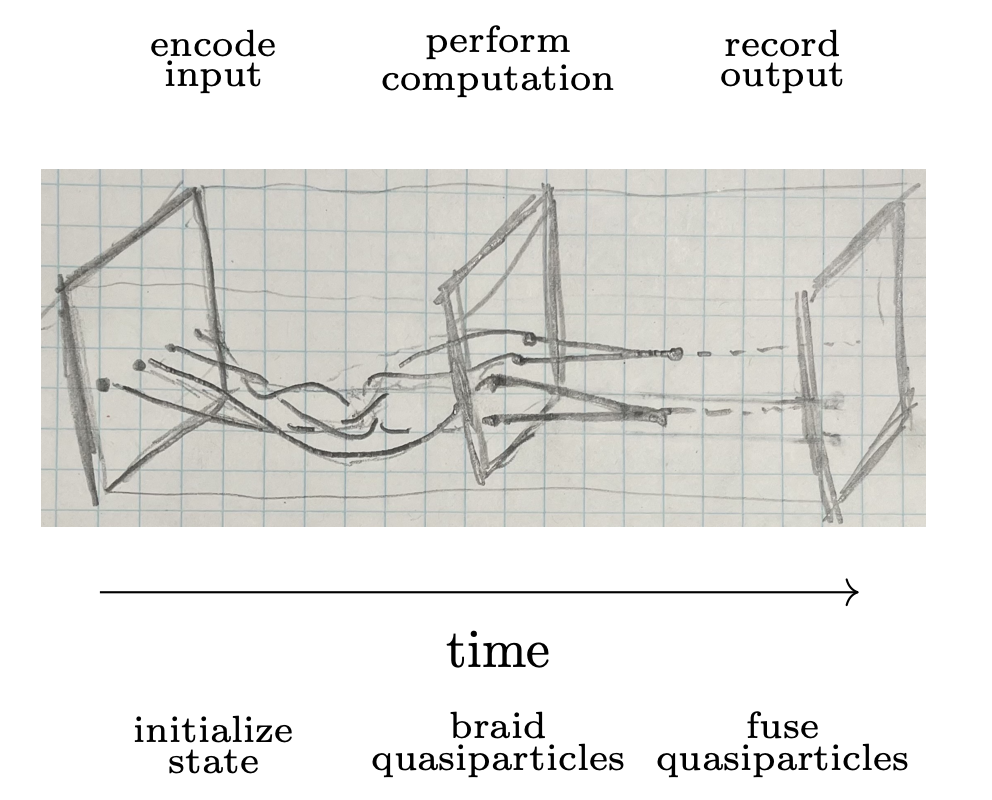
\includegraphics[scale=0.35]{TQC-outline}
\caption{A schematic of topological quantum computing}
\label{fig:TQC-outline}
\end{center}
\end{figure}

To make the above discussion more concrete, we will give a worked example. In this example we use a specific topological order known as the \textit{Fibonacci particle theory} to run Shor’s efficient quantum factorization algorithm \cite{shor1994algorithms}. The input of Shor’s algorithm is a positive integer. The output of Shor’s algorithm is the factorization of that integer. Shor’s algorithm is \textit{efficient} in the sense that it uses polynomially many quantum logic gates to arrive at its answer relative to the size of the input. Throughout this passage we will use \textit{efficient} and \textit{polynomially sized} interchangeably. The Fibonacci particle theory is a specific topological order, which describes in an algebraic fashion how the overall state changes when quasiparticles are braided and fused.

The first step in running Shor’s algorithm on a Fibonacci quantum computer is to translate the positive integer input into a certain braid. This is done using an efficient classical algorithm. The second step is to run this braid on a Fibonacci quantum computer. This is done by initializing some prescribed state and then braiding its quasiparticles. This initialization and braiding is performed repeatedly, and after every time two of the quasiparticles are fused. This gives us a real number, which is the probability that the two quasiparticles annihilate after the braiding. An efficient classical algorithm is then used to take this real number and obtain from it the factorization of the original input. Since all of these steps are efficient, it gives a topological quantum algorithm for factoring integers. The schematic for this process is shown below:

\begin{equation*}
\tikzfig{shor-fibonacci}
\end{equation*}

The magic in the above procedure is the existence of these two classical algorithms: a first one for encoding integers into braids and a second one for decoding real numbers into factorizations. These algorithms are nontrivial. They are due to Freedman-Larsen-Kitaev-Wang \cite{freedman2002modular}. In fact, Freedman-Larsen-Kitaev-Wang showed that any problem which can be efficiently solved using a quantum circuit can also be solved using the Fibonacci particle theory, via a similar method of efficient classical preprocessing and postprocessing. It is in this sense that the Fibonacci theory is \textit{universal} for quantum computation.

The final step of this process would be to create a physical topological system which is described by the Fibonacci theory, which would serve as our quantum computer. In the realm of materials, the most promising approach seems to be to use specially tuned versions of the fractional quantum Hall system \cite{zhu2015fractional}. While these materials are theorized to host quasiparticles described by the Fibonacci theory, the difficulty of the experiment makes them inaccessible to current technology. There has been progress made on topological quantum error correcting codes which work by simulating the Fibonacci theory \cite{schotte2022quantum, schotte2022fault}. However these codes at the current moment have structural issues and require an unbearable amount of overhead to run, making them unfeasible to use on modern computers.

Progress on topological quantum computing has thus been focused on realizing topological particle theories other than the Fibonacci theory. These other theories can be constructed in more workable materials, and can be simulated as topological quantum error correcting codes with less overhead. The drawback of these other theories is that they are typically less computationally powerful, meaning that they require more tricks and techniques to achieve universal quantum computing. There are a great number of different proposals for how to achieve universal topological quantum computing, based on different particle theories, different methods of encoding information, different methods of manipulating information, and different methods of reading out information. It is an exciting time to be a theorist in the field of topological quantum information.

\subsubsection{Defects in ordered media}

We will now work through a complete mathematical example of a family of topological systems. Our examples will be \textit{classical} topological systems. Many of the important subtlties of topological quantum information are already present in the classical case. Topological classical information is a smaller subject than topological quantum information - the reader should have a relatively complete grasp of the subject by the end of the chapter. Much of the discussion in this chapter is taken from an excellent review article by Mermin \cite{mermin1979topological}. The goal of this chapter is both to give a family of relevant examples to the reader, as well as to give a crash-course on the relevant topology.

The family of systems we will describe goes by many names. In communities of experimentally focused physicists it goes by the name \textit{ordered media}. In mathematical physics communities it goes by the name \textit{classical gauge theory}. In pure mathematics it would be described as \textit{homotopy theory}. We will construct a system based on every topological space $M$. We will call $M$ the order space of our theory.

To describe a system in physics, the first step is to define the space of possible states of the system. In this case, states will correspond to \textit{continuous maps $\phi: \RR^2\to M$}. We now give physical intuition for this choice of state space. The choice of $\RR^2$ as a source represents the underlying material. We are working on an infinite flat plane. Describing a function $\phi: \RR^2\to M$ amounts to choosing a value $\phi(x)$ for every point $x\in \RR^2$. In this way we imagine our system as being made up of infinitely many objects, one placed at each point in $\RR^2$, each of which has an internal state space $M$. The fact that $\phi$ must be continuous is a compatibility condition between the states of the objects at nearby points. It says that nearby objects must have similar states. We now list some examples:

\begin{itemize}
\item \textbf{Classical XY model of a 2D electron gas}. In this example, $M$ is the circle. An electron can be modeled as a point particle with a magnetic dipole pointing in some direction. This magnetic dipole is known as the \textit{spin} of the election, and can point in any direction in the plane. The topological space of all possible directions in the plane is a circle. The fact that nearby electrons must have similar spins is known as Hund’s rule, and is the most fundamental incarnation of ferromagnetism. It is physically derived as a consequence of the Pauli exclusion principle.

\item \textbf{A-phase of superfluid Helium-3}.  [WORK: fill in example]

\item \textbf{Biaxial nematics}. In this example, $M$ is a certain quotient of the special orthogonal group $\SO(3)$ of rotations in three dimensional space. The objects at every point in the biaxial nematic should be thought of as small rectangles with unequal side lengths. These rectangles can be oriented in any direction in three dimensional space. In practice these objects will often be molecular compounds. They will not be exactly rectangular, but have the same symmetry group as a rectangle which is enough for the model to be accurate. To compute the space of possible orientations of a small rectangle, we work by the method of symmetries. Choosing some reference orientation to start with, every rotation in three dimensional space brings the rectangles to new orientations. The space of orientations of the rectangle is hence equal to $\SO(3)$ modulo the rotations which fix the rectangle. That is, $M$ is equal to $\SO(3)$ modulo the symmetry group of a rectangle. [WORK: Talk to someone who knows about biaxial nematics. What's with the continuity condition? How does this work, really?]
\end{itemize}

We will now analyze these systems. In doing this analysis we will want to use the ideas of \textit{deformation} and \textit{topological equivalence}. Of course, these ideas are vague and require rigorous notions to make precise. We define these notions now.

\begin{definition}
Let $X,Y$ be topological spaces, and let $f,g: X\to Y$ be continuous maps. A \textbf{homotopy} between $f$ and $g$ is a map $H: X\times [0,1] \to Y$ such that $H(x, 0)=f(x)$ and $H(x,1)=g(x)$ for all $x\in X$.
\end{definition}

The idea is that the maps $H(\cdot,t):X\to $Y for $t\in [0,1]$ are a continuously deforming family. The first map $H(\cdot, 0)$ is equal to $f$, and as $t$ moves forward the maps $H(\cdot,t)$ slowly change until at $t=1$ they become $H(\cdot,1)=g$. If there exists a homotopy between two maps, then we say those maps are \textit{homotopic}. It is straightforward to verify that homotopy is an equivalence relation (see Exercise [ref]). More colloquially, if $f$ and $g$ are homotopic we say that $f$ can be deformed into $g$. This is our relevant notation of topological equivalence.

We can use homotopies to get a picture of dynamics in our system. We call continuous maps $H: \RR^2 \times \RR_{\geq 0}\to M$ \textit{time evolutions} of the system. The map $\phi_t=H(\cdot,t): \RR^2\to M$ is called \textit{the state of the system at time $t$}. For every $T>0$, the map $H_T:\RR^2\times [0,1]\to M$ given by $H_T(x,t)=H(x,t\cdot T)$ gives a homotopy between $\phi_0$ and $\phi_T$. Hence, the states of the system at various times are all homotopic. In this sense the system is \textit{evolving by homotopies}. The following proposition is an important part of understanding the nature of the system:

\begin{proposition}
Let $M$ be a path connected topological space. Every pair of continuous maps $\phi_0,\phi_1:\RR^2\to M$ is homotopic.
\end{proposition}
\begin{proof}
Consider the map $H_0: \RR^2\times [0,1]\to M$ given by $H_0(x,t)=\phi_0(tx)$. Since multiplication in $\RR^2$ is continuous, $H_0$ is continuous. Hence, $H_0$ gives a homotopy between the constant map $H_0(\cdot,0)=\phi_0(0)$ and $H_0(\cdot,1)=\phi_0(x)$. Similarly, the map $H_1:\RR^2\times [0,1]\to M$  given by $H_1(x,t)=\phi_1(tx)$ gives a homotopy between the constant map $H_1(\cdot,0)=\phi_1(0)$ and $H_1(\cdot,1)=\phi_1(x)$.

Now, since $M$ is path connected, there exists a continuous map $\ell: [0,1]\to M$ such that $\ell(0)=\phi_0(0)$ and $\ell(1)=\phi_1(0)$. Thus, the map $H_\ell:\RR^2\times [0,1]\to M$ given by $H_\ell(x,t)=\ell(t)$ establishes a homotopy between the constant maps $H_\ell(\cdot,0)=\phi_0(0)$ and $H_\ell(\cdot,1)=\phi_1(0)$. Composing the homotopies from $\phi_0(x)$ to $\phi_0(0)$, $\phi_0(0)$ to $\phi_1(0)$, and $\phi_1(0)$ to $\phi_1(x)$, we arrive at a homotopy between $\phi_0(x)$ and $\phi_1(x)$ as desired.
\end{proof}

The above proposition can be interpreted as saying that as our system evolves in time, we can expect it to go from any state to any other state. In other words, all of the possible states of our system are topologically equivalent and hence it contains \textit{no topologically invariant information}. This means that we will need to add more complexity to the system before we can study topological information.

This complexity will come from introducing quasiparticles. These quasiparticles go by many names. In the theory of ordered media they are known as defects. In gauge theory they are known as particles. In homotopy theory they are known as point singularities. For the sake of brevity, we will use the term defect. A defect is a point at which we will drop our condition that the state $\phi:\RR^2\to M$ be continuous. This is done by making $\phi$ \textit{undefined} at certain points. Our new system is called \textit{ordered media with finitely many defects}. The state space consists of pairs $(S,\phi)$, where $S\subset \RR^2$ is a finite set and $\phi: \RR^2\\ S\to M$ is a continuous map.

Dynamics in our new system can involve the movement of defects. Let $\gamma_1… \gamma_n: \RR_{\geq 0} \to \RR^2$ be continuous maps, with $ \gamma_i(t)\neq \gamma_j(t)$ for all $i\neq j$, $t\in [0,1]$. These maps represent the trajectories of the defects, subject to the condition that no two defects collide. Continuous maps

$$H:\RR^2\times \RR_{\geq 0} \backslash \bigcup_{t\geq 0}\bigcup_{i=1}^{n}(\gamma_i(t),t)\to M$$

represent dynamics in our system. We call such maps \textit{defect-mobile homotopies}. At every time $t\geq 0$, the system is in the $n$-defect state

$$\phi_t=H(\cdot,t): \RR^2\backslash \bigcup_{i=1}^{n}\gamma_i(t)\to M.$$

. If the trajectories $\gamma_i$ are constant with respect to $t$ for all $i$, we will call $H$ a \textit{defect-fixed homotopy}. This now leads us to two immediate questions:

\begin{enumerate}
\item What information is invariant under defect-mobie homotopy?
\item What information is invariant under defect-fixed homotopy?
\end{enumerate}

After answering these questions, we will move on to building a computer based on defects in ordered media. The idea is that our computer will store its information within attributes of the state which are invariant under defect-fixed homotopy. These attributes, typically, will \textit{not} be invariant under defect-mobile homotopy. This means that if defects are braided around eaech other, the values of these defect-fixed attributes will change. This change in information is a \textit{computation}. This leads to two more central questions:

\begin{enumerate}
\setcounter{enumi}{2}
\item How does braiding affect defect-fixed information?
\item Which choices of order  space $M$ make for effective computers?
\end{enumerate}

Answering these questions requires a detailed analyis of our model using techniques from homotopy theory.

\subsubsection{The fundamental group}

In this subsection we analyse defects in ordered media using the \textit{fundamental group} from homotopy theory. Readers familiar with homotopy theory should familiarize themselves with the statement of Proposition [ref] before moving on to the next subsection. We begin with some terminology and basic results - we will return to ordered media breifly.

\begin{definition} Let $X$ be a topological space.
\begin{itemize}
\item A continuous map $\gamma:[0,1]\to X$ is called a \textbf{path} in $X$ from $\gamma(0)$ to $\gamma(1)$;
\item Given two paths $\gamma_0,\gamma_1$ with the same start and end points, a \textbf{path homotopy} from $\gamma_0$ to $\gamma_1$ is a map $H:[0,1]\times [0,1]\to X$ such that $H(\cdot,0)=\gamma_0$, $H(\cdot,1)=\gamma_1$, $H(0,t)=\gamma_0(0)=\gamma_1(0)$, and $H(1,t)=\gamma_0(1)=\gamma_1(1)$ for all $t\in [0,1]$.
\item A \textbf{loop} is a path with the same start and end point. This common start and end point is called the \textbf{base point} of the loop.
\item Given a point $x\in X$, the \textbf{fundamental group of $X$ based at $x$} is defined as a set to be the collection of equivalence classes of loops in $X$ based at $x$ up to path homotopy. It is denoted $\pi_1(X,x)$.
\end{itemize}
\end{definition}

The term fundamental \textit{group} is justified by the following proposition:

\begin{proposition} Let $X$ be a topological space, and let $x\in X$ be a point. We define a binary operation on the space of loops in $X$ based at $x$ by the formula 

$$(\alpha_0\cdot \alpha_1)(t)=
\begin{cases}
\alpha_0(2t) & 0\leq t < 1/2\\
\alpha_1(2t-1) & 1/2\leq t \leq 1
\end{cases}$$

for all loops $\alpha_0,\alpha_1$ based at $x$. This binary operation induces a well-defined map path homotopy equivalence classes, yielding a binary operation on $\pi_1(X,x)$. This binary operation endows $\pi_1(X,x)$ with the structure of a group.
\end{proposition}
\begin{proof}.[WORK: do proof]
\end{proof}

We now prove some basic results about the fundamental group:

\begin{proposition} Let $X$ be a topological space, and let $x\in X$ be a point.
\begin{enumerate}[(a)]
\item Let $\gamma:[0,1]\to X$ be a path. Given every loop $\alpha$ in $X$ based at $\gamma(0)$, define the map

$$i_\gamma(\alpha)(t)=
\begin{cases}
\gamma(1-3t) & 0\leq t < 1/3 \\
\alpha(3t-1) & 1/3 \leq t <2/3 \\
\gamma(3t-2) & 2/3 \leq t \leq 1
\end{cases}$$

to be a loop based at $\gamma(1)$. This assignment induces a well defined map on path homotopy equivalence classes. Moreover, the induced map

\begin{equation*}
i_\gamma: \pi_1(X,\gamma(0))\xrightarrow{}\pi_1(X,\gamma(1))
\end{equation*}

is an isomorphism of groups.

\item Let $S^1$ be the circle, which we define as the interval $[0,1]$ with $0$ and $1$ identified. Every loop in $X$ induces a map from the circle to $X$, by gluing $0$ and $1$. This natural map induces a \textbf{bijection} between conjugacy classes in the fundamental group and homotopy classes of maps from the circle to $X$.

\end{enumerate}
\end{proposition}
\begin{proof}. [WORK: do proof]
\end{proof}

The fundamental group of the order space $M$ will play an important role in our analysis of the system. Hence, we will now compute the fundamental groups of the order spaces corresponding to the xy model of an electron gas, the A-phase of superfluid helium, and biaxial nematics:

\begin{proposition}$\,$
\label{fundamental-group-computations}
\begin{enumerate}[(a)]
\item $\pi_1(S^1,x)\cong \ZZ$ for all $x\in S^1$;
\item $\pi_1(\RR^2\backslash S,x)\cong\Free(S)$ for all finite sets $S\subset \RR^2$ and $x\in \RR^2\backslash S$, where $\Free(S)$ denotes the free group with generators corresponding to elements of $S$.
\item .[WORK: compute superfluid helium example];
\item .[WORK: compure biaxial nematics example];
\item For all groups $G$, there exists a topological space $X$ such that $\pi_1(X,x)\cong G$ for all $x\in X$.
\end{enumerate}
\end{proposition}
\begin{proof}.[WORK: do proof]
\end{proof}

As a consequence of proposition \ref{fundamental-group-computations}(a), we can define the notion of \textit{winding number}.

\begin{corollary} Choose $b,x\in \RR^2$. We have a canonical isomorphism of groups $\pi_1(\RR^2\backslash \{x\},b)\cong \ZZ$. Given a loop $\alpha:[0,1]\to U\backslash \{x\}$ based at $b$, the integer corresponding to the element $[\alpha]\in \pi_1(U\backslash \{x\},b)$ is called the \textbf{winding number of $\alpha$ around $x$}. It is denoted $\wind(\alpha,x)$.
\end{corollary}
\begin{proof}.[WORK: do proof]
\end{proof}

We are now ready to return to our analysis of defects in ordered media. Let $(S,\phi)$ be a state in an ordered media with order space $M$. Suppose $S=\{x_1, ...x_n\}$, and choose a basepoint $b\in \RR^2\backslash S$. For all $1\leq i\leq n$, define loops $\alpha_i$ based at $b$ which go around $x_i$ exactly once counterclockwise, and do not wind around any of the other $x_j$. Formally, this amounts to choosing $\alpha_i$ so that

$$\wind(\alpha_i,x_j)=
\begin{cases}
1 & i=j\\
0 & \text{otherwise}.
\end{cases}$$

Each map $\alpha_i$ can be postcomposed with $\phi$ to give a map $(\phi\circ \alpha_i): [0,1]\to M$. In this way, every loop in phtsical space can be pushed forward to a loop in order space. The important feature to notice is that as $\phi$ changes by homotopies, the map $\phi\circ \alpha_i$ changes by homotopies. Additionally, as $\alpha_i$ changes by homotopies, the map $\phi\circ \alpha_i$ changes by homotopies. In this way, the homotopy class of $\phi\circ \alpha_i$ as a map from the circle to $M$ is an invariant of $\phi$ which is invariant under defect-mobile homotopy. Moreover, Proposition [ref](b) implies that all maps which wind exactly once around $\alpha_i$ and wind zero times around the other $\alpha_j$ are homotopic [WORK: this is false]. Hence, the value of the invaraint does not depend on the choice of $\alpha_i$. By Proposition [ref](b), homotopy classes of loops in order space correspond to conjugacy classes in $\pi_1(M,m)$ for any fixed $m\in M$. Hence, we conclude that associated to every defect in $\phi$, there is a corresponding conjugacy class in $\pi_1(M,m)$ for any fixed $m\in M$. This conjugacy class is an invariant under defect-mobile homotopy.

All of the path homotopy classes of maps $\phi\circ \alpha_i$ give elements of $\pi_1(M,\phi(b))$. It is natural to ask why these elements are not invariants under defect-mobile homotopies, but only their conjugacy class. The answer is twofold:

\begin{enumerate}
\item As $\phi$ changes by homotopies, $\phi(b)$ can change. This movement of basepoint will affect the path homotopy class of $\phi\circ \alpha_i$.
\item As the state changes under defect mobile homotopy, another defect $x_j$ could pass through $\alpha_i$. At this point, the composition $\phi\circ \alpha_i$ becomes \textit{undefined}. The homotopy classes of $\phi\circ \alpha_i$ before and after $x_j$ moves through it could be different. Choosing $\alpha_i$ smaller so that $x_j$ does not pass through it is possible, but this might neccecarily involve changing the basepoint of $\alpha_i$. This change in basepoint. will affect the path homotopy class of $\phi\circ \alpha_i$. [WORK: add picture]
\end{enumerate}

Under defect-fixed homotopy, the concern (2) dissapears. Moreover, if we add the technical condition that $\phi(b)$ cannot change during the defect-fixed homotopy then the concern (1) will dissapear as well. Hence, the elements $\pi_1(M,\phi(b))$ are invariants under basepoint-preserving defect-fixed homotopies. If the basepoint is allowed to vary it will change all of the path homotopy classes at once. This brings us to our main result of the subsection, which gives a full classification of information stored within defects in ordered media:

\begin{proposition} Let $M$ be a path connected topological space. Let $S=\{x_1...x_n\}$ be a finite set, and let $\phi:\RR^2 \backslash S\to M$ be a continuous map. Let $\alpha_i$ be loops in $\RR^2\backslash S$ based at $b\in \RR^2\backslash S$ such that

$$\wind(\alpha_i,x_j)=
\begin{cases}
1 & i=j\\
0 & \text{otherwise}.
\end{cases}$$

\begin{enumerate}[(a)]
\item The homotopy classes $[\phi\circ \alpha_i]$ of maps $S^1\to M$ do not depend on the choice of $\alpha_i$. These homotopy classes are invariants under defect-mobile homotopy.
\item The path homotopy classes of $[\phi\circ \alpha_i]\in \pi_1(M,\phi(b))$ do not depend on the choice of $\alpha_i$. These path homotopy classes are invariant under defect-fixed homotpies which preserve the value of $\phi(b)$. These invariants establish a bijection

$$\left(\substack{\text{states $(S,\phi)$ up to} \\ \text{basepoint-preserving defect-fixed homotopy}}\right)\xrightarrow{\sim} \prod_{i=1}^n\pi_1(M,\phi(b))$$

\item The element $\left([\phi\circ\alpha_i]\right)_{i=1}^n \in \prod_{i=1}^n\pi_1(M,\phi(b))$ does not depend on the choice of $\alpha_i$. This establishes a bijection [WORK: state this correctly - it should be simultanous conjugation by an element of $\pi_1(M,\phi(b))$]

$$\left(\substack{\text{states $(S,\phi)$ up to} \\ \text{defect-fixed homotopy}}\right)\xrightarrow{\sim} \left(\text{conjugacy classes in }\prod_{i=1}^n\pi_1(M,\phi(b))\right)$$
\end{enumerate}
\end{proposition}
\begin{proof}.[WORK: do proof]
\end{proof}

[WORK: there IS some dependence on the $\alpha_i$]

\subsubsection{Topological classical computation}

Our goal in this section is to make a topological computer. Throughout this section we will fix some notation. We let $M$ be a path connected topological space, we let $S=\{x_1, ...x_n\}$ be a finite set, we let $\phi:\RR^2\backslash S\to M$ be a state, and we let $b\in \RR^2\backslash S$, $m\in M$ be basepoints. Throughout this section we will assume that $\phi(b)=m$ is \textit{fixed}. This is mainly a matter of convenience - allowing it to move would require a tedious amount of digressions about conjugacy classes. Physically, this can be justified by pushing the basepoint away towards infinity where it cannot be disturbed.

Proposition [ref] tells us that basepoint-preserving defect-fixed homotopy classes of states correspond to elements of $\prod_{i=1}^n\pi_1(M,m)$. It is in this product that we will store our information. For example, if $\pi_1(M,m)\cong \ZZ_2$ then $\prod_{i=1}^n\pi_1(M,m)=\prod_{i=1}^n\ZZ_2$ is an $n$-bit string. More generally, one will need to outline some encoding method for converting standard information storage formats into elements of $\prod_{i=1}^n\pi_1(M,m)$.

The general picture to have in mind is that of an experimenter who has control over the trajectories of defects, but no control over the specifics of the map $\phi$ in the bulk. The goal is to engineer a protocol by which every map $f:\prod_{i=1}^n\pi_1(M,m)\to\prod_{i=1}^n\pi_1(M,m)$ can be realized by braiding defects around each other.

Let $S'=\{x_1', ...x_n'\}$ be another finite set. Let $\gamma_1..\gamma_n$ be paths in $\RR^2$ such that $\gamma_i(0)=x_i$, $\gamma_i(1)=x_i'$, $\gamma_i(t)\neq b$, and $\gamma_i(t)\neq \gamma_j(t)$ for all $i\neq j$, and $t\in [0,1]$.

As the defects in $S$ move along the paths $(\gamma_i)_{i=1}^n$, the overall state of the system will change. This will allow us to perform computations. An important feature is that the way the state of the system will change will not depend on the specifics of the trajectories $(\gamma_i)_{i=1}^n$ that are picked. If collection of paths $(\gamma_i)_{i=1}^n$ is distored a small amount this will not change the computation. Of course, what it means for the collection of paths to be distored is a technical mathematical notion. We will define it now:

\begin{definition} Let $X$ and $Y$ be topological spaces. Let $f_0,f_1: X\to Y$ be continuous injective functions. An \textbf{ambient isotopy} from $f_0$ to $f_1$ is a map $H: Y\times [0,1]\to Y$ such that $H(\cdot,t)$ is a homeomorphism for all $t\in [0,1]$, $H(\cdot,0)$ is the identity map, and $H(\cdot,1)\circ f_0=f_1$.
\end{definition}

We say that two collections of paths $(\gamma_i)_{i=1}^n$ are ambient isotopic if their corresponding maps

\begin{align*}
\{1...n\}\times [0,1]&\to \RR^2 \times [0,1]\\
(i,t)&\mapsto (\gamma_i(t),t)
\end{align*}

are ambient isotopic [WORK: this is wrong - this definition doesnt preserve the endpoints of the braids]. The following proposition gives us a description of what happens when the defects are moved along the paths $\gamma_i$:

\begin{proposition} Let $S,S',(\gamma_i)_{i=1}^n$ be as above. Let $\phi:\RR^2\backslash S \to M$ be a continuous map. There exists a basepoint-preserving defect-mobie homotopy

$$H:\RR^2\times \RR_{\geq 0} \backslash \bigcup_{t\geq 0}\bigcup_{i=1}^{n}(\gamma_i(t),t)\to M$$

such that $H(\cdot,0)=\phi$. The basepoint-preserving defect-fixed homotopy class of $H(\cdot,1)$ depends only on the choice of $(\gamma_i)_{i=1}^n$, and not on the choice of $H$. Moreover, the basepoint-preserving defect-fixed homotopy class of $H(\cdot,1)$ depends only on the choice of $(\gamma_i)_{i=1}^n$ up to ambient isotopy.

\end{proposition}
\begin{proof}.[WORK: do proof]
\end{proof}

The above proposition motivates the fact that the space of collections of paths $(\gamma_i)_{i=1}^n$ up to ambient isotopy will be important for computation. We introduce notation to make our discussion simpler:

\begin{definition} Let $S=\{x_1...x_n\} \subset \RR^2$ be a finite set. The space of all collections of paths $(\gamma_i)_{i=1}^n$ in $\RR^2$ such that $\{\gamma_i(0)\}_{i=1}^n=\{\gamma_i(1)\}_{i=1}^n$ as sets and $\gamma_i(t)\neq \gamma_j(t)$ for all $i\neq j$ and $t\in [0,1]$ up to ambient isotopy is known as the \textbf{braid group} of $S$. It is denoted $B_S$. Elements of the braid group are known as \textbf{braids}. The paths $\gamma_i$ are known as the \textbf{strands} of the braid. If $\gamma_i(0)=\gamma_i(1)$ for all $1\leq i\leq n$, then we say that $\left[(\gamma_i)_{i=1}^n\right]$ is \textbf{pure braid}. The set of pure braids on $S$ is called the pure braid group, and is denoted $P_S$.
\end{definition}

As promised by the nomenclature, the braid group and the pure braid group are both groups:

\begin{proposition} Let $S\subset \RR^2$ be a finite set. Let $\beta=\left[(\gamma_i)_{i=1}^n\right]$ and $\beta'=\left[(\gamma_i')_{i=1}^n\right]$ be two braids in $B_S$. Define a permutation $\sigma: \{1...n\}\to \{1...n\}$ by the property that

$$\gamma_i(1)=\gamma_{\sigma(i)}(0).$$

Define a binary operation on $B_S$ by the formula

$$\beta \cdot \beta' = \left[\left(\gamma_i \cdot \gamma_{\sigma(i)}'\right)_{i=1}^n\right].$$

This is a well defined binary operation, and induces a group structure on $B_S$. The above assignment of braids to permutations induces a surjective homomorphism of groups $B_S\to \Sym_n$, where $\Sym_n$ is the $n$-letter symmetric group. The kernel of this homomorphism is the pure braid group $P_S$. This gives a short exact sequence

$$0\to P_n\to B_n\to \Sym_n\to 0$$
\end{proposition}
\begin{proof}.[WORK: do proof]
\end{proof}

For the sake of convenience, we will assume that none of the trajectories in any of our braids pass through our base point $b\in \RR^2$. We can now reinterpret Proposition [ref] in the language of algebra:

\begin{proposition} Let $\beta\in B_S$ be braid. Define a map

$$\rho_S:B_S\to \Sym\left(\prod_{i=1}^n\pi_1(M,m)\right)$$

 as follows. Let $\phi:\RR^2\backslash S\to M$ be a state. Let $H$ be a defect-mobile homotopy whose defects move along some representative of $\beta$, and satisfies the initial condition $H(\cdot,0)=\phi$. We set $\rho_S([\phi])=[H(\cdot,1)]$, where the basepoint-preserving defect-mobile homotopy classes $[\phi]$ and $[H(\cdot,1)]$ are identified with elements of $\prod_{i=1}^n\pi_1(M,m)$ by Proposition [ref]. This is a well-defined homomorphism of groups.
\end{proposition}
\begin{proof}.[WORK: do proof]
\end{proof}

Understanding topological classical computation amounts to understanding the structure of the braid groups, and the structure of the homomorphisms $\rho$ of Proposition [ref]. Performing this analysis is much simpler when all of the defects are in a standard position. Hence, throughout the rest of this subsection we will let $S=\{(0,1), (0,2)...(0,n)\}$. In this case we denote $B_S$ by $B_n$, and refer to it as the \textit{$n$-strand braid group}. We will denote the corresponding $\rho_S$ by $\rho_n$. [WORK: where is $b$? What choices of $\alpha_i$ do we make?]

The most basic braid arrises by swapping adjacent defects. Explicitely, for $1\leq i\leq n-1$, we denote by $\sigma_i$ the braid which acts by the identity on all $(0,j)$ with $j\neq i, i+1$ and swaps $(0,i)$ and $(0,i+1)$, with $(0,i)$ going below $(0,i+1)$. This can be paramaterized by making $\gamma_i$ a unit semicircle in the lowerhalf plane and $\gamma_{i+1}$ a unit semicirlce in the upperhalf plane. These swaps form the basic logical gates which will build up all our computations. The following proposition describes their algebraic properties, and how they act under $\rho$:

\begin{proposition} The following facts about the braid group are true:

\begin{enumerate}
\item The braids $\sigma_1...\sigma_{n-1}$ generate $B_n$;
\item The relations $\sigma_i\sigma_{i+1}\sigma_i=\sigma_{i+1}\sigma_{i}\sigma_{i+1}$ and $\sigma_{i}\sigma_{j}=\sigma_{j}\sigma_{i}$ hold for all $1\leq i,j \leq n-1$, $|i-j|\geq 2$. Moreover, these relations are sufficient to generate all relations on the braid group;
\item $\rho_n(\sigma_i)$ is the map $\prod_{i=1}^n\pi_1(M,m)\to\prod_{i=1}^n\pi_1(M,m)$ which sends $(g_1...g_n)$ to 

$$(g_1,g_2... g_{i+1},g_{i+1}^{-1}g_ig_{i+1} ... g_n)$$
\end{enumerate}

\end{proposition}
\begin{proof}.[WORK: do proof]
\end{proof}

With this algebraic description of the braid group,

[WORK: BIG PROBLEM!!!!!! We still need to introduce creating defect/antidefect pairs. I think that I might need to rethink this rigorous approach.... ]

$\newline\newline$

\large \textbf{Exercises}:\normalsize

\begin{enumerate}[\thesection .1.]

\item .[WORK: show that simulability => \textit{efficient} simulability. Do the work in the case $G=A_5$]

\item .[WORK: maybe show that nilpotent => polynomial growth?]

\end{enumerate}

\section{Quantum mechanics}

\subsection{Overview}

\subsubsection{Introduction}

In this chapter we will give an introduction to quantum mechanics. The goal of this book is to give an exposition of topological quantum information. So far we have described topological \textit{classical} information - all that's missing now is quantum mechanics!

One of the difficulties of working with quantum mechanics is that it is physically unintuitive. Conversely, one of the advantages of working with quantum mechanics is that it is mathematically basic. Quantum mechanics is mathematically enitirely described by linear algebra. The mathematical intricacies of quantum mechanics often arrise from complications from working in infintie dimensional spaces. In topological quanum information, however, all of the spaces of interest are finite dimensional and hence the mathematics involved is quite straightforward. In this chapter we will give a dictionary between the physical language of quantum mechanics and the mathematical language of linear algebra.

Quantum mechanics is typically used to describe small object. A natural question is \textit{why(?)}. If quantum mechanics is correct, then it should equally welll apply to small and large objects. The answer to this question is subtle, and brings us to back to the thesis of this book.

Large scale macroscopic phenomina are emergent from coherent small scale microscopic phenomina. Here, the word \textit{coherent} is used very intentionally. It is used to mean ``held together", ``integrated", or ``organized". The fact that collections of microscopic quantum degrees of freedom fail to form macroscopic quantum degrees of freedom is known as \textit{decoherence}. It is the ubiquity of decoherence which makes are macroscopic world seem classical.

It is exactly for this reason that topological quantum systems are so special. They are essentially unique in the fact that they can cohrently hold quantum information at macroscopic length and time scales. This is because decoherence is caused by repeated noise from the environment, which corrupts fragile quantum information. Topological quantum systems are defined by their stored information is not affected by local changes. Hence, if noise is sufficiently local and sufficiently controlled, the information in topological systems will remain coherent. 

This makes topological quantum matter a fantastic place to first learn quantum theory. The mathematics is simple because all spaces involved are finite dimensional, and the quantum effects are more dominant than in almost any other macroscopic phenomina!

\subsubsection{Experimental motivation}

Before diving into a formal treatment of quantum mechanics, let us first motivate why quantum mechanics has to be like it is. The most famous aspect of quantum mechanics is its probabilistic nature. As Einstein famously said, \textit{``God does not play dice"}. If quantum mechanics was just probabilistic, however, it wouldn't bother physicists nearly as much at it does. Quantum mechanics is a sort of twisted probability theory:

\begin{quote}
``What happens if you try to come up with a theory that's \textit{like} probability theory, but based on the $2$-norm instead of the $1$-norm?... Quantum mechanics is what inevitably results." - Scott Aaronson\footnote{Page 112 of Aaronson's ``Quantum Computing since Democritus" \cite{aaronson2013quantum}}
\end{quote}

Throughout this introduction to quantum mechanics we will take the lens of comparing quantum mechanics with classical probability theory. Some properties of quantum mechanics, like \textit{superposition} and \textit{entanglement}, are already clearly present in the world of probability. Other properties, like \textit{interference}, are not. To make this clear, we will present a few experiements which demonstrate the proabilistic nature of quantum mechanics, and the ways in which quantum mechanics goes beyond probability theory.

[WORK: which experiments should I chose? Double slit? Polarized light? Pairs of entangled photos? It would be cool to get experiments which are relevant to topological matter if possible. It would also be cool to get experiments which almost immediately motivate the exact form of quantum mechanics. I'm not a physicist though - need to get someone else more knowledgable to make this section.]

\subsection{Axiomatic development}

\subsubsection{Probability theory}

Seeing as quantum mechanics is a modified probability theory, before axiomatizing quantum mechanics we will first axiomatize probability theory in terms of linear algebra. The goal is to highlight what an axiomatization of a physical theory should look like, so that the jump to quantum mechanics is as predictable as possible.

Intuitively, we all know what probability theory is. We start with some set $S$ which represents the possible outcomes of our probability theory. States in probability theory are probability distributions on $S$. That is, assights of probabilities (positive real numbers) to each elements of $S$ such that the total probability is $1$. We will focus entirely on \textit{finite} probability spaces. This greatly simplifies our analysis. Finite probability spaces require only basic linear algebra to describe, wheras infinite probability spaces requires measure theory.

For example, suppose we are flipping a coin. The space of possible outcomes is $S=\{h,t\}$, heads or tails. A fair coin flip would have $50\%=1/2$ probability of giving heads, and $50\%=1/2$ probability of giving tails.

A convement notation for proability distribution is the language of weighted sums. The state $\sum_{x\in S}p_x\ket{x}$ denotes the state with probability $p_x\geq 0$ of having outcome $\left| x\right>$, where $\sum_{x\in S}p_x=1$. In the case of heads and tais, we would write

$$\ket{\text{fair flip}}\coloneqq\frac{1}{2}\ket{h}+\frac{1}{2}\ket{t}.$$

The notation $\ket{\cdot}$ for states is known as a \textit{ket}. This is part of so-called \textit{Dirac notation}, which is widespread in quantum theory. We use it here to help ease our transition from probability theory to quantum mechancis.

Mathematically, a formal sum is an element of a vector space. That is, the weighted sums corresponding to probability distributions are elements of the vector space

$$\RR[S]\coloneqq \text{span} \left\{\left.\ket{x}\right| x\in S\right\}.$$

For convenience, we will refer to elements of $\RR[S]$ of the form $\sum_{x\in S}p_x \ket{x}$ with $p_x\geq 0$, $\sum_{x\in S}p_x=1$ as \textit{normalized vectors}. Our disucssion can be summarized as saying that probability distributions on $S$ correspond to normalized vectors in $\RR[S]$.

We now move on to discussing the way that probability spaces can evolve, or be related to one another. Certainly, a relation between a probability space with outcomes $S$ and a probability space with outcomes $S'$ will be some function

$$\left(\text{normalized vectors in }\RR[S]\right)\xrightarrow{}\left(\text{normalized vectors in }\RR[S']\right)$$

which gives a rule for going from proability distrubutions on $S$ to probability distributions on $S'$. However, not every function will give a valid assignment. For example, suppose we are studying the outcomes of lottery tickets. Ticket 1 has an $80\%$ chance of being a winner, and Ticket 2 has a $40\%$ of being a winner. You haven't scratched your ticket all the way yet, so you have a $50\%$ chance of having Ticket 1 and a $50\%$ chance of having Ticket 2. What is the probability that you win the lottery? The standard way of computing it would be as follows:

\begin{align*}
\text{result}(\ket{\text{your ticket}})&=\text{result}\left(\frac{1}{2}\ket{\text{Ticket 1}}+\frac{1}{2}\ket{\text{Ticket 2}})\right)\\
&=\frac{1}{2}\text{result}(\ket{\text{Ticket 1}})+\frac{1}{2}\text{result}(\ket{\text{Ticket 2}})\\
&=\frac{1}{2}\left(\frac{4}{5}\ket{\text{win}}+\frac{1}{5}\ket{\text{lose}}\right)+\frac{1}{2}\left(\frac{2}{5}\ket{\text{win}}+\frac{3}{5}\ket{\text{lose}}\right)\\
&=\frac{3}{5}\ket{\text{win}}+\frac{2}{5}\ket{\text{lose}}.
\end{align*}

Hence, you have a $3/5=60\%$ chance of winning. The key insight in this computation was that probabilistic processes are \textit{linear}. That is, ``$\text{result}$" induces a linear map between $\RR[\{\text{Ticket 1}, \text{Ticket 2}\}]$ and $\RR[\text{win},\text{lose}]$. More generally, given finite sets $S,S'$ any linear map $\RR[S]\to\RR[S']$ which sends normalized vectors to normalized vectors could represent some valid probabilistic process.

The final topic to tackle before giving the full axiomatization is the question of \textit{joining} probabilitstic systems. In this book we will mostly be constructing systems out of a lot of smaller consitutent parts, so the question of fitting together smaller systems to make one larger system is of utmost importance. Suppose we have two smaller systems with possible outcomes $S$, $S'$. To describe a state in the joined system, it is neccecary and sufficient to describe how that state restricts to each subsystem. In this way, possible outcomes of the joined system will correspond to pairs $(x,x')$ where $x\in S$ is the portion of the overall state in $S$ and $x'\in S'$ is the portion of the overall state in $S'$. This means the space out outcomes in the joined system is the Cartesian product $S\times S'$.

We are now ready to state the full axioms of probability theory:

\begin{definition}[Axioms of probability theory] $\,$

\begin{enumerate}
\item (Systems) A probabilistic system is a real vector space of the form $\RR[S]$, where $S$ is a finite set. The normalized vectors in $\RR[S]$ correspond to probability distributions on $S$.
\item (Processes) A probabilistic process going from a system $S$ to a system $S'$ is a linear map $\RR[S]\to \RR[S']$, which sends normalized vectors to normalized vectors.
\item (Joining systems) If $S$ and $S'$ are two finite sets, the system obtained by joining $\RR[S]$ and $\RR[S']$ is $\RR[S\times S']$.
\item (Measuring systems) Given a normalized vector $\sum_{x\in S}p_x \left |x\right>\in \RR[S]$, measurement corresponds to collapsing onto an outcome, where we collapse into each $x\in S$ with probability $p_x$.
\end{enumerate}

\raggedleft\qedsymbol{}
\end{definition}

\subsubsection{Basis-dependent quantum mechanics}

The basis-dependent version of quantum mechanics can be estblished by copying the axioms of probability theory almost verbatim, replacing the 1-norm with the 2-norm.

Given a finite set $S$, a normalized vector in $\RR[S]$ is one of the form $\sum_{x\in S}p_x \ket{x}$, where $p_x\geq 0$ and $\sum_{x\in S}p_x=1$.  This quantity $\sum_{x\in S}p_x$ is known as the \textit{1-norm} of the vector $p=(p_x)_{x\in S}$.

In quantum mechanics we re-define the notation of normalized vector. A normalized vector in quantum mechanics is a state $\sum_{x\in S}c_x \ket{x}$, where $c_x\in \CC$ are arbitary complex numbers and $\sum_{x\in S}|c_x|^2=1$. The sum of norm-squares $\sum_{x\in S}|c_x|^2$ is known as the \textit{2-norm} of the vector $c=(c_x)_{x\in S}$. In this way, the norm-squares $|c_x|^2$ form a probility distrubution on $S$.

Thus, given some finite set $S$, states in the quantum system based on $S$ correspond to normalized vectors in $\CC[S]$. As a matter of convention, normalized vectors in $\RR[S]$ will always refer to the 1-norm definition and normalized vectors in $\CC[S]$ will always refer to the 2-norm definition. We are now ready to state the basic axioms of quantum theory:

\begin{definition}[Axioms of quantum mechanics, version 1] $\,$

\begin{enumerate}
\item (Systems) A quantum system is a complex vector space of the form $\CC[S]$, where $S$ is a finite set. The normalized vectors in $\CC[S]$ correspond to quantum states on $S$. Here, a \textit{normalized} vector $v=\sum_{x\in S}c_x\left|x\right>$ is one for which $\sum_{x\in S}|c_x|^2=1$, where $|c_x|^2$ denotes the norm square.
\item (Processes) A quantum process going from a system $S$ to a system $S'$ is a linear map $\CC[S]\to \CC[S']$ which sends normalized vectors to normalized vectors.
\item (Joining systems) If $S$ and $S'$ are two finite sets, the system obtained by joining $\CC[S]$ and $\CC[S']$ is $\CC[S\times S']$.
\item (Measuring systems) Given a normalized vector $\sum_{x\in S}c_x \left |x\right>\in \CC[S]$, measurement corresponds to collapsing into a pure state, where we collapse into each $x\in S$ with probability $|c_x|^2$.
\end{enumerate}

\raggedleft\qedsymbol{}
\end{definition}

We now relate these axioms to the previous dicussion, and introduce terminology. The formal sums $\sum_{x\in S}c_x\ket{x}$ are no probability distributions. They are called \textit{wavefunctions}. Every state in quantum mechanics is encoded in a wavefunction. Treating the possible outcomes in $S$ as positions of the wavefunction, we get the analogy

\begin{itemize}
\item Wave = multiple possible positions, spread-out =$\sum_{x\in S}c_x\ket{x}\in \CC[S]$;
\item Particle = single positions, definite = $\left|x\right>$, $x\in S$.
\end{itemize}

By axiom (4), measuring of wavefunction collapses into into a single particle. This is the essence of wave-particle duality in quantum mechanics. The numbers $c_x$ are not probilities. They are called \textit{amplitudes}. If a state $\ket{\psi}=\sum_{x\in S}c_x \ket{x}$ has non-zero aplidue at $x,y\in S$, then we say that $\ket{\psi}$ is in a \textit{superposition} of being in state $\ket{x}$ and $\ket{y}$.

Within this framework it is easy to demonstrate the phenominon of interference. Define the transformation $M: \CC[S]\to \CC[S]$ by

$$M(\0)=\frac{1}{\sqrt{2}}\0+\frac{1}{\sqrt{2}}\1,$$

$$M(\1)=\frac{1}{\sqrt{2}}\0-\frac{1}{\sqrt{2}}\1.$$

Applying $M$ to $\0$ and measuring gives $0$ and $1$ with equal probability, and same with applying $M$ to $\1$. When we apply $M$ to the equal superposition of $0$ and $1$, however, this results in the state

$$H\left(\frac{1}{\sqrt{2}}\0+\frac{1}{\sqrt{2}}\1\right)=\frac{1}{\sqrt{2}}\left(\frac{1}{\sqrt{2}}\0+\frac{1}{\sqrt{2}}\1\right)+\frac{1}{\sqrt{2}}\left(\frac{1}{\sqrt{2}}\0-\frac{1}{\sqrt{2}}\1\right)=\0.$$

We can summarize this as saying that there was \textit{constructive interference} in the $\0$, and \textit{destructive interference} in the $\1$. The amplitudes had the same signs in the $\0$ causing the probability of measuring $0$ to add, and the amplitudes had opposite signs in the $\1$, causing the probabilities of measuring $1$ to cancel. 





\subsubsection{Basis-independent quantum mechanics}

\subsection{Secondary structures}

\subsubsection{Entanglement and incomplete measurements}

\subsubsection{Hamiltonians and the Schrodinger equation}

\subsection{Computational complexity}

\subsubsection{Classical computation}

\subsubsection{Probabilistic computation}

\subsubsection{Quantum computation}

[WORK: add a history section]


$\newline\newline$

\large \textbf{Exercises}:\normalsize

\begin{enumerate}[\thesection .1.]

\item hey
\end{enumerate}

\section{Topological quantum order}

\section{Category theory}

[WORK: use probability spaces and quantum spaces as examples of categories!]

\section{Topological quantum field theory}

\section{Modular tensor categories}

\section{Topological quantum computation}

\section{Further structure}
\bibliographystyle{alpha}
\bibliography{ref}


\end{document}






